\documentclass[conference]{IEEEtran}
\IEEEoverridecommandlockouts
% The preceding line is only needed to identify funding in the first footnote. If that is unneeded, please comment it out.
\usepackage{cite}
\usepackage{amsmath,amssymb,amsfonts}
\usepackage{algorithmic}
\usepackage{graphicx}
\usepackage{textcomp}
\usepackage{xcolor}
\usepackage{caption}
\usepackage{subcaption}
\usepackage{array}

\usepackage{mathtools} 

%added by Ye
\usepackage{fontspec}

%for typing Myanmar text, you can also used with Myanmar3 font
\newfontfamily {\padauktext}[Script=Myanmar]{Padauk}
%\newfontinstance {\padauktext}[Script=Myanmar]{Padauk}

%for double quote
\newcommand{\quotes}[1]{``#1''}
%added by Ye

\def\BibTeX{{\rm B\kern-.05em{\sc i\kern-.025em b}\kern-.08em
    T\kern-.1667em\lower.7ex\hbox{E}\kern-.125emX}}
\begin{document}

\title{Statistical Machine Translation \\between Kachin and Rawang}

\author{\IEEEauthorblockN{1\textsuperscript{st} Ye Kyaw Thu}
\IEEEauthorblockA{\textit{Language and Semantic Technology Research Team (LST)} \\
\textit{National Electronics and Computer Technology Center (NECTEC)}\\
PathumThani, Thailand \\
ka2pluskha2@gmail.com}
\and
\IEEEauthorblockN{2\textsuperscript{nd} Manar Hti Seng}
\IEEEauthorblockA{\textit{Faculty of Computer Science} \\
\textit{University of Computer Studies (Banmaw)}\\
Banmaw, Myanmar \\
junjasmine298@gmail.com}
\and
\IEEEauthorblockN{3\textsuperscript{rd} Thazin Myint Oo}
\IEEEauthorblockA{\textit{Natural Language Process Lab.} \\
\textit{University of Computer Studies, Yangon (UCSY)}\\
Yangon, Myanmar \\
thazinmyintoo@ucsy.edu.mm}
\and
\IEEEauthorblockN{4\textsuperscript{th} Dee Wom}
\IEEEauthorblockA{\textit{Faculty of Computer Science} \\
\textit{University of Computer Studies (Banmaw)}\\
Banmaw, Myanmar \\
Mgnyochaw7@gmail.com}
\and
\IEEEauthorblockN{5\textsuperscript{th} Hpau Myang Thint Nu}
\IEEEauthorblockA{\textit{Faculty of Computer Science} \\
\textit{University of Computer Studies (Banmaw)}\\
Banmaw, Myanmar \\
thintnuhpaumyang@gmail.com}
\and
\IEEEauthorblockN{6\textsuperscript{th} Seng Mai}
\IEEEauthorblockA{\textit{Faculty of Computer Science} \\
\textit{University of Computer Studies (Banmaw)}\\
Banmaw, Myanmar \\
sarinaryuri@gmail.com}
\and
\IEEEauthorblockN{7\textsuperscript{th} Thepchai Supnithi}
\IEEEauthorblockA{\textit{Language and Semantic Technology Research Team (LST)} \\
\textit{National Electronics and Computer Technology Center (NECTEC)}\\
PathumThani, Thailand \\
thepchai@gmail.com}
\and
\IEEEauthorblockN{8\textsuperscript{th} Khin Mar Soe}
\IEEEauthorblockA{\textit{Natural Language Process Lab.} \\
\textit{University of Computer Studies, Yangon (UCSY)}\\
Yangon, Myanmar \\
khinmarsoe@ucsy.edu.mm}
}

\maketitle

\begin{abstract}
This paper contributes the first evaluation of the quality of machine translation between Kachin and Rawang. We also developed a Kachin-Rawang parallel corpus (around 10K sentences) based on the Myanmar language of ASEAN MT corpus. The 10 folds cross-validation experiments were carried out using three different statistical machine translation approaches: phrase-based, hierarchical phrase-based, and the operation sequence model (OSM). The results show that all three statistical machine translation approaches give higher and comparable BLEU and RIBES scores for both Kachin to Rawang and Rawang to Kachin machine translations. OSM approach achieved the highest BLEU and RIBES scores among three approaches machine translation.\end{abstract}

\begin{IEEEkeywords}
Statistical Machine Translation, Under-resourced languages, Dialects, Kachin, Rawang
\end{IEEEkeywords}

\section{Introduction}
Our main motivation for this research is to investigate SMT performance for Kachin and Rawang language pair. The Kachin language is closely related to Rawang language and it is often considered as dialect of Kachin language. The state-of-the-art techniques of statistical machine translation (SMT) [1], [2] demonstrate good performance on translation of languages with relatively similar word orders [3]. 
To date, there have been some studies on the SMT of Myanmar language. Ye Kyaw Thu et al. (2016) [4] presented the first large-scale study of the translation of the Myanmar language. A total of 40 language pairs were used in the study that included languages both similar and fundamentally different from Myanmar. The results show that the hierarchical phrase-based SMT (HPBSMT) [5] approach gave the highest translation quality in terms of both the BLEU [6] and RIBES scores [7].  Win Pa Pa et al (2016) [8] presented the first comparative study of five major machine translation approaches applied to low-resource languages. PBSMT, HPBSMT, tree-to-string (T2S), string-to-tree (S2T) and OSM translation methods to the translation of limited quantities of travel domain data between English and {Thai, Laos, Myanmar} in both directions. The experimental results indicate that in terms of adequacy (as measured by BLEU score), the PBSMT approach produced the highest quality translations. Here, the annotated tree is used only for English language for S2T and T2S experiments. This is because there is no publicly available tree parser for Lao, Myanmar and Thai languages. According to our knowledge, there is no publicly available tree parser for both Kachin and Rawang languages and thus we cannot apply S2T and T2S approaches for Kachin-Rawang language pair. From their RIBES scores, we noticed that OSM approach achieved best machine translation performance for Myanmar to English translation. Moreover, we learned that OSM approach gave highest translation performance between Khmer (the official language of Cambodia) and twenty other languages, in both directions [9].

Relating to Myanmar langauge dialects, Thazin Myint Oo  et al. (2018) \cite{b25} contributed the first PBSMT, HPBSMT and OSM machine translation evaluations between Myanmar and Rakhine. The experiment was used the 18K Myanmar-Rakhine parallel corpus that constructed to analyze the behavior of a dialectal Myanmar-Rakhine machine translation. The results showed that higher BLEU (57.88  for Myanmar-Rakhine and 60.86 for Rakhine-Myanmar) and RIBES (0.9085 for Myanmar-Rakhine and 0.9239 for Rakhine-Myanmar) scores can be achieved for Rakhine-Myanmar language pair even with the limited data. Based on the experimental results of previous works, in this paper, the machine translation experiments between Kachin and Rawang were carried out using PBSMT, HPBSMT and OSM.

\section{Related Work}
Karima Meftouh et al. built PADIC (Parallel Arabic Dialect Corpus) corpus from scratch, then conducted experiments on cross dialect Arabic machine translation [10].  PADIC is composed of dialects from both the Maghreb and the Middle-East. Some interesting results were achieved even with the limited corpora of 6,400 parallel sentences.
	Using SMT for dialectal varieties usually suffers from data sparsity, but combining word-level and character-level models can yield good results even with small training data by exploiting the relative proximity between the two varieties [11]. Friedrich Neubarth et al. described a specific problem and its solution, arising with the translation between standard Austrian German and Viennese dialect. They used hybrid approach of rule-based preprocessing and PBSMT for getting better performance.
	Pierre-Edouard Honnet et al. proposed solutions for the machine translation of a family of dialects, Swiss German, for which parallel corpora are scarce [12]. They presented three strategies for normalizing Swiss German input in order to address the regional and spelling diversity. The results show that character-based neural MT was the most promising one for text normalization and that in combination with PBSMT achieved 36\% BLEU score.

\section{Kachin State and Kachin People}
The Kachin State is situated in north Myanmar and is the place where the most of jinghpaw peoples live in. It lies between north latitude 23°27'and 28°25' longitude 96°0' and 98°44'. The area of Kachin State is 89,041km (34,379 sq mi). The capital of Kachin State is Myitkyina and Bhamo is the second largest historic city of jinghpaw peoples. About 2 millions of jinghpaw peoples live in Myanmar. In jinghpaw, there are two groups called Bhamo jinghpaw and Myitkyina jinghpaw. Jinghpaw peoples also live in Shan State. Jinghpaw peoples are on of  the ethnic groups in Myanmar. Jinghpaw comprises six tribes or subdivisions: Lisu, Lashi, Rawang, Zaiwa, Lhao Vo. All have their own language and literature. As they all comes from Jinghpaw, they can also speak or use the Jinghpaw language. Jinghpaw alphabet is based on Lathin script. The Jinghpaw literature was strated using in the era of “King Min Done Min” (1853-1878). However, the literature that Kachin peoples are using now was  written on May 5,1895 by Dr. Ola Hanson, in the era of “King Thi Paul” (1878-1885) .

\section{Kachin and Rawang Languages}
\label{sec:KachinLanguage}
\subsection{Kachin or Jingpho Language}
\label{subsec:KachinOrJingpho}
Jingpho (Jinghpaw, Chingp'o) or Kachin (Burmese: {\padauktext ကချင်ဘာသာ} [kətɕɪ̀ɴ bàðà]) is a Tibeto-Burman language of the Sal branch mainly spoken in Kachin State, Burma and Yunnan, China. There are a lot of meanings for Jingpho. In the Jingpho language, Jingpho means people. The term "Kachin language" can refer either to the Jingpho language or to a group of languages spoken by various ethnic groups in the same region as Jingpo: Lisu, Lashi, Rawang, Zaiwa, Lhao Vo, Achang and Jingpho. These languages are from distinct branches of the highest level of the Tibeto-Burman family. The Jingpho alphabet is based on the Latin script. The ethnic Jingpho (or Kachin) are the primary speakers of Jingpho language, numbering approximately 900,000 speakers. The Turung of Assam in India speak a Jingpho dialect with many Assamese loanwords, called Singpho.

\subsection{Rawang Language}
\label{subsec:RawangLanguage}
Rawang peoples is the sub-group of Kachin (Jinghpaw) in Myanmar. Rawang peoples live in northern Kachin state: Puato, Machanbaw, Naungmaw, Kawnglangphu, and Pannandin townships. 70,000 of Rawang people live in Myanmar. There are four enthic roup in Rawang. They are Lungmi, Matwang, Daru and  Tangsar. The Normal ( - ) , High ( ´ ) and Low ( ` ) symbols:

\subsection{Grammar of Myanmar, Kachin and Rawang}
\label{subsecsec:Grammar}

Kachin and Rawang sentences use several punctuation symbols \quotes{.}, \quotes{,}, \quotes{?},  \quotes{“} , \quotes{”}, \quotes{‘}, \quotes{’},\quotes{!}, \quotes{:}, \quotes{;} and \quotes{-}. Myanmar (my), Kachin (kc) and Rawang (rw) languages have same word order (i.e. Subject, Object and Verb). Some example of parallel sentences in Myanmar(my), Kachin(kc) and Rawang(rw) are as follows :\\

\noindent my: {\padauktext နေကောင်းလား ။}\\
kc:  Hkam kaja ai i .\\
rw: PÀMVRÀ ÍÈ MÁ .\\

\noindent my: {\padauktext  လုံချည် တစ်ထည် ဘယ်လောက်လဲ ။}\\
kc:  Ba hkang langai  kade rai ?\\
rw: SHVRØM TÌQ DUNG KÀDVNGTĒ ÍÈ lĒ .\\

\noindent my: {\padauktext  ထမင်းစား ပြီးပြီ လား ။}\\
kc:  Shat   sha  sai i ?\\
rw: VMPÀ VM BØĪ MÁ .\\

\noindent my: {\padauktext ကလေးများ ကစား နေကြသည် ။}\\
kc:  Ma ni  gasup taw nga ma ai .\\
rw: CVMRE RĪ GVSØP MĒ .\\

\section{Methodology}
\label{sec:Method}
In this section, we describe the methodology used in the machine translation experiments for this paper.

\begin{figure*}[ht!]
%\begin{center}
  \centering
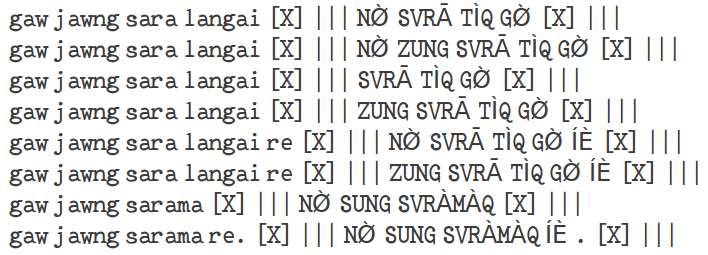
\includegraphics[width=0.7\textwidth]{./fig/kc-rw-hpbsmt-phrase-table.png}
  \caption{Some examples of hierarchical phrase-based grammar between Kachin and Rawang phrases}
%\end{center}
\label{fig:hpbsmtFig}
\end{figure*}

\subsection {Phrase-Based Statistical Machine Translation}
\label{subsec:PBSMT}
A PBSMT translation model is based on phrasal units \cite{b1}. Here, a phrase is simply a contiguous sequence of words and generally, not a linguistically motivated phrase. A phrase-based translation model typically gives better translation performance than word-based models. We can describe a simple phrase-based translation model consisting of phrase-pair probabilities extracted from corpus and a basic reordering model, and an algorithm to extract the phrases to build a phrase-table \cite{b14}. 
The phrase translation model is based on noisy channel model. To find best translation $ \Hat{e} $ 
that maximizes the translation probability $ \mathbf{P}(f) $ given the source sentences; mathematically. Here, the source language is French and the target language is an English. The translation of a French sentence  into an English sentence  is modeled as equation~\ref{eq:1}.

\begin{equation} \label{eq:1}
\Hat{e}=argmax_e \mathbf {P}(e|f)
\end{equation}
Applying the Bayes’ rule, we can factorized into three parts.
\begin{equation} \label{eq:2}
P(e|f)=\frac{\mathbf{P}(e)}{\mathbf{P}(f)}\mathbf{P}(f|e)
\end{equation}
The final mathematical formulation of phrase-based model is  as follows:
\begin{equation} \label{eq:3}
argmax_e \mathbf {P}(e|f)=argmax_e \mathbf {P}(f|e) \mathbf{P}(e)
\end{equation}

We note that denominator $\mathbf{P}(f)$ can be dropped because for all translations the probability of the source sentence remains the same. The $\mathbf {P}(e|f)$ variable can be viewed as the bilingual dictionary with probabilities attached to each entry to the dictionary (phrase table). The $\mathbf{P}(e)$ variable governs the grammaticality of the translation and we model it using n-gram language model under the PBMT paradigm.

\subsection {Hierarchical Phrase-Based Statistical Machine Translation}
\label{subsec:HPBSMT}

The hierarchical phrase-based SMT approach  is a model based on synchronous context-free grammar \cite{b14}. The model is able to be learned from a corpus of unannotated parallel text. The advantage this technique offers over the phrase-based approach is that the hierarchical structure is able to represent the word re-ordering process. The re-ordering is represented explicitly rather than encoded into a lexicalized re-ordering model (commonly used in purely phrase-based approaches). This makes the approach particularly applicable to language pairs that require long-distance re-ordering during the translation process \cite{b15}. Some examples of hierarchical phrase based grammar between Dawei and Myanmar phrases are shown in Figure~\ref{fig:hpbsmtFig}.


\subsection {Operation Sequence Model}
\label{subsec:OSM}

The operation sequence model which combines the benefits of two state-of-the-art SMT frameworks named n-gram-based SMT and phrase-based SMT. This model simultaneously generate source and target units and does not have spurious ambiguity that is based on minimal translation units \cite{b16} \cite{b17}. It is a bilingual language model that also integrates reordering information. OSM motivates better reordering mechanism that uniformly handles local and non-local reordering and strong coupling of lexical generation and reordering. It means that OSM can handle both short and long distance reordering. The operation types are such as generate, insert gap, jump back and jump forward which perform the actual reordering. The following shows an example translation process of English sentence \quotes{Please sit here} into Myanmar language with the OSM.\\

\noindent Source: Please sit here\\
Target: {\padauktext ကျေးဇူးပြုပြီး ဒီမှာ ထိုင် }\\

\begin{description}
   \item Operation 1: Generate (Please, {\padauktext ကျေးဇူးပြုပြီး})
   \item Operation 2: Insert Gap
   \item Operation 3: Generate (here, {\padauktext ကျေးဇူးပြုပြီး ဒီမှာ})
   \item Operation 4: Jump Back (1)
   \item Operation 5: Generate (sit, {\padauktext ကျေးဇူးပြုပြီး ဒီမှာ ထိုင် })
\end{description}

\section{Experiment}
\label{sec:Exp}

\subsection {Corpus Statistics}
\label{subsec:Corpus}

We used 10K Myanmar sentences (without name entity tags) of the ASEAN-MT Parallel Corpus \cite{b18}, which is a parallel corpus in the travel domain. It contains six main categories and they are people (greeting, introduction and communication), survival (transportation, accommodation and finance), food (food, beverage and restaurant), fun (recreation, traveling, shopping and nightlife), resource (number, time and accuracy), special needs (emergency and health). Manual translation to Kachin and Rawang was done manually. We held 10-fold cross-validation experiments and used 8,468 to 8,519 sentences for training, 500 sentences for development and 985 to 1,026 sentences for evaluation respectively.

\subsection {Moses SMT System}
\label{subsec:Moses}
We used the PBSMT, HPBSMT and OSM system provided by the Moses toolkit \cite{b19} for training the PBSMT, HPBSMT and OSM statistical machine translation systems. The word segmented source language was aligned with the word segmented target language using GIZA\ensuremath{++} \cite{b20}. The alignment was symmetrized by grow-diag-final and heuristic [1]. The lexicalized reordering model was trained with the msd-bidirectional-fe option \cite{b21}. We use KenLM \cite{b22} for training the 5-gram language model with modified Kneser-Ney discounting \cite{b23}. Minimum error rate training (MERT) \cite{b24} was used to tune the decoder parameters and the decoding was done using the Moses decoder (version 2.1.1). We used default settings of Moses for all experiments.

\section{Evaluation}
\label{sec:Evaluation}
We used two automatic criteria for the evaluation of the machine translation output. One was the de facto standard automatic evaluation metric Bilingual Evaluation Understudy (BLEU) \cite{b6} and the other was the Rank-based Intuitive Bilingual Evaluation Measure (RIBES) \cite{b7}.  The BLEU score measures the precision of n-gram (over all n ≤ 4 in our case) with respect to a reference translation with a penalty for short translations \cite{b6}. Intuitively, the BLEU score measures the adequacy of the translation and large BLEU scores are better. RIBES is an automatic evaluation metric based on rank correlation coefficients modified with precision and special care is paid to word order of the translation results. The RIBES score is suitable for distance language pairs such as Myanmar and English. Large RIBES scores are better.

\section{Results and Discussion}
\label{sec:R&D}

The BLEU and RIBES score results for machine translation experiments with PBSMT, HPBSMT and OSM are shown in Table 1. Bold numbers indicate the highest scores among three SMT approaches. The RIBES scores are inside the round brackets. Here, “kc” stands for Kachin, “rw” stands for Rawang, “src” stands for source language and “tgt” stands for target language respectively.


\begin{table*}[h!]
\caption{\label{table:result} Average BLEU and RIBES scores for PBSMT, HPBSMT and OSM}
\begin{center}
%\begin{tabular}{ |C|C|C|C| } 
\begin{tabular}{ |c|c|c|c| } 
 \hline
 \bf src-tgt & \bf PBSMT & \bf HPBSMT & \bf OSM \\[5pt]
 \hline
 kc-rw & 43.071 (0.79964) & 43.197 (0.80064) & \bf 43.973 \bf (0.80079)\\[5pt] 
 \hline
 rw-kc & 46.281 (0.81064) & 46.129 (0.81224) & \bf 46.597 \bf (0.81180)\\[5pt]
 \hline
\end{tabular}
\end{center}
\end{table*}


%The BLEU and RIBES score results for machine translation experiments with PBSMT, HPBSMT and OSM between Kachin and Rawang languages are shown in Table 1. 
From the results, OSM method achieved the highest BLEU and RIBES score for both Kachin to Rawang and Rawang to Kachin bi-directional machine translations. Interestingly, the BLEU and RIBES score of all three methods are comparable performance. Our results with current parallel corpus indicate that Rawang to Kachin machine translation is better performance (around 3 BLEU and 0.02 RIBES scores higher) than Kachin to Rawang machine translation direction. 

As we expected, generally, machine translation performance of all three SMT approaches between Kachin and Rawang languages achieved good scores for both BLEU and RIBES. The reason is that as we mentioned in Section ~\ref{subsec:KachinOrJingpho} and  Section~\ref{subsec:RawangLanguage}, the two languages, Kachin and Rawang are close languages.  We assume that long distance reordering is relatively rare and only local reordering is enough for the Kachin-Rawang language pair.

\section{Error Analysis}
\label{sec:errorAnalysis}

We also used the SCLITE (score speech recognition system output) program from the NIST scoring toolkit SCTK version 2.4.10 \cite{b26} for making dynamic programming based alignments between reference and hypothesis
strings for detail analysis on translation errors (WER: Word Error Rate). The formula for WER can be stated as equation~\ref{eq:4}:

\begin{equation} \label{eq:4}
WER=(I+D+S)100/N
\end{equation}

where $S$ is the number of substitutions, $D$ is the number of deletions, $I$ is the number of insertions, $C$ is the number of correct words and $N$ is the number of words in the reference ($N=S+D+C$). Note that if the number of insertions is very high, the WER can be greater than 100\%. Table~\ref{table:WER}  present the WER percentages of translation between Kachin and Rawang. Note that this WER table is calculated based on one experimental result of the 10-fold cross validation. Table~\ref{table:WER} shows that HPBSMT gave the lowest WER (41.6\%) for Kachin-Rawang translation and OSM gave the lowest WER (41.1\%) for Rawang-Kachin translation.

%The results show that syllable segmentation gave the lowest WER values for Transformer and CNN models and the difference is higher for the SentencePiece segmentation for both MWT-MSL and MSL-MWT translation tasks (see Figure 3 and 4).

\begin{table*}[h!]
\caption{\label{table:WER} Average WER\% for PBSMT, HPBSMT and OSM with around 1,000 sentences (lower is better)}
\begin{center}
%\begin{tabular}{ |C|C|C|C| } 
\begin{tabular}{ |c|c|c|c| } 
 \hline
 \bf src-tgt & \bf PBSMT & \bf HPBSMT & \bf OSM \\[5pt]
 \hline
 kc-rw & 42.5\% & \bf 41.6\% & 42.7\%\\[5pt] 
 \hline
 rw-kc & 43.6\% & 42.6\% & \bf 41.1\%\\[5pt]
 \hline
\end{tabular}
\end{center}
\end{table*}

From our studies, the top 10 confusion matrixes for Kachin-Rawang and Rawang-Kachin OSM machine translation can be seen in Table~\ref{table:KachinRawangCM} and Table~\ref{table:RawangKachinCM}.
%The word error rate (WER) is 43.8\%.

\begin{table}[h!]
\caption{\label{table:KachinRawangCM} The top 10 confusion pairs of OSM model for Kachin-Rawang machine translation}

\begin{center}
\begin{tabular}{ |c|c| } 
 \hline
 \bf Freq & \bf Reference ==> Hypothesis \\ [5pt]
 \hline
 33  & wĒ ==> yÀ \\[5pt]
 \hline
 26  & yÀ ==> wĒ \\[5pt]
 \hline
 19  & lÓ ==> ÍÈ \\[5pt]
 \hline
 12  &  chvng ==> gwĪn\\[5pt]
 \hline
 10  & Ē ==> ngĒ\\[5pt]
 \hline
 9  & ÍÈ ==> Ē\\[5pt]
 \hline
 8  & . ==> ?\\[5pt]
 \hline
 8  & kŪ ==> wĒ\\[5pt]
 \hline
 7  & ? ==> .\\[5pt]
 \hline
 7  & gwĪn ==> bvtgwĪn\\[5pt]
 \hline
\end{tabular}
\end{center}
\end{table}

\begin{table}[h!]
\caption{\label{table:RawangKachinCM} The top 10 confusion pairs of OSM model for Rawang-Kachin machine translation}

\begin{center}
\begin{tabular}{ |c|c| } 
 \hline
 \bf Freq & \bf Reference ==> Hypothesis \\ [5pt]
 \hline
 13  & u. ==> ai. \\[5pt]
 \hline
 12  & ai ==> le \\[5pt]
 \hline
 11  & . ==> ai. \\[5pt]
 \hline
 11  & ai. ==> . \\[5pt]
 \hline
 10  & ai ==> na \\[5pt]
 \hline
 10  & ai. ==> re. \\[5pt]
 \hline
 9  & na ==> ai \\[5pt]
 \hline
 8  & le ==> ai \\[5pt]
 \hline
 7  & ai. ==> rai? \\[5pt]
 \hline
 7  & ai. ==> sai. \\[5pt]
 \hline
\end{tabular}
\end{center}
\end{table}

We also made manual error analysis on translated outputs of the best OSM model, and we found that dominant errors are different in sentence level. The followings are some common translation error patterns for PBSMT, HPBSMT and OSM: \\
%We will introduce four frequent error patterns and they are \enquotes{Male-Female Vocabulary Error}, \enquote{Paraphrasing Error}, \enquote{Word Segmentation Error} and \enquote{Negative Error}. The followings are some example translation mistakes for each category:

% Male-Female Error
%\begin{center} \textbf{\#\#\# Male-Female Vocabulary Error \#\#\#}  \\ \end{center}

\begin{center} \textbf{\#\#\# PBSMT, Kachin-Rawang \#\#\#}  \\ \end{center}
%PBSMT
%SOURCE: {\textbf{xx xx xx}}  \\
\noindent No. [1]\\
\noindent Scores: (\#C \#S \#D \#I) 7 3 2 1\\
REF:  NÀ Í    NGÀ *** LVP KÀQ GØ̀ DĒDVM  MÁ RÀ Ē YO . \\
HYP:  NÀ NØ̀ NGÀ YÀ LVP KÀQ ***** NØ̀NT NA   RÀ Ē ** . \\
Eval:     S          I            D     S       S          D   \\

%SOURCE: {\textbf{xx xx xx}}  \\
\noindent No. [2]\\
\noindent Scores: (\#C \#S \#D \#I) 5 2 1 0\\
REF:  WĒ MÉ NØ̀ BVTGWĪN TÌQ CHVNG MV:Ī . \\
HYP:  YÀ MÉ ***** BVTGWĪN TÌQ GWĪN MV:Ī . \\
Eval: S       D                   S  \\

\begin{center} \textbf{\#\#\# HPBSMT, Kachin-Rawang \#\#\#}  \\ \end{center}
%HPBSMT
%SOURCE: {\textbf{xx xx xx}}  \\
\noindent No. [3]\\
\noindent Scores: (\#C \#S \#D \#I) 2 4 2 0\\
REF:  Àng YØP BǾĪ WĒ  Í  NÀ ÍÈ .\\ 
HYP:  Àng **** ***** SHÀ YUP Ē  LĒ  .\\ 
Eval:      D    D     S    S   S   S \\

%SOURCE: {\textbf{xx xx xx}}  \\
\noindent No. [4]\\
\noindent Scores: (\#C \#S \#D \#I) 3 5 1 0\\
REF:  ÀNG MÀQ VNÍ GØ     KARØT SHVJVNG SHĪ Ē  . \\
HYP:  ÀNG **** VNÍ SANHTAI WÀ    SHAMAN  VL   LĒ . \\
Eval:      D         S       S      S       S    S \\

%OSM, kc-rw
\begin{center} \textbf{\#\#\# OSM, Kachin-Rawang \#\#\#}  \\ \end{center}

%SOURCE: {\textbf{xx xx xx}}  \\
\noindent No. [5]\\
\noindent Scores: (\#C \#S \#D \#I) 6 1 0 1\\
REF:  SHǾNGTØ̀NG RĪ ***** KĀDVNG TØ̀NG ÍÈ LĒ . \\
HYP:  TØ̀NG       RĪ NØ̀ KĀDVNG TØ̀NG ÍÈ LĒ . \\
Eval:  S                 I   \\
 
\hfill \break
%SOURCE: {\textbf{xx xx xx}}  \\
\noindent No. [6]\\
\noindent Scores: (\#C \#S \#D \#I) 7 0 0 1\\
REF:  YÀ MÉ NØ̀ NGÀ *** SHÀ LŌ . \\
HYP:  YÀ MÉ NØ̀ NGÀ YÀ SHÀ LŌ . \\
Eval:                    I \\

\begin{center} \textbf{\#\#\# PBSMT, Rawang-Kachin \#\#\#}  \\ \end{center}

%SOURCE: {\textbf{xx xx xx}}  \\
\noindent No. [7]\\
\noindent Scores: (\#C \#S \#D \#I) 2 0 0 2\\
REF:  nyau langai *** ** \\
HYP:  nyau langai SHA GA \\
Eval:             I   I\\

%SOURCE: {\textbf{xx xx xx}}  \\
\noindent No. [8]\\
\noindent Scores: (\#C \#S \#D \#I) 4 0 2 0\\
REF:  dai GAW yakhkak NGA ai i? \\
HYP:  dai *** yakhkak *** ai i? \\
Eval:     D           D  \\

\begin{center} \textbf{\#\#\# HPBSMT, Rawang-Kachin \#\#\#}  \\ \end{center}

%SOURCE: {\textbf{xx xx xx}}  \\
\noindent No. [9]\\
\noindent Scores: (\#C \#S \#D \#I) 4 1 0 1\\
REF:  ngai gaw mi mi ** RE. \\
HYP:  ngai gaw mi mi RE AI. \\
Eval:                I  S  \\

%SOURCE: {\textbf{xx xx xx}}  \\
\noindent No. [10]\\
\noindent Scores: (\#C \#S \#D \#I) 4 2 0 1\\
REF:  dai BALL PEN   langai re ** i? \\
HYP:  dai GAW  KUMGA langai re AI i? \\
Eval:     S    S               I  \\

\begin{center} \textbf{\#\#\# OSM, Rawang-Kachin \#\#\#}  \\ \end{center}

%SOURCE: {\textbf{xx xx xx}}  \\
\noindent No. [11]\\
\noindent Scores: (\#C \#S \#D \#I) 6 1 0 3\\
REF:  * dai gaw *** HKAGAWM langai re *** ai i? \\
HYP:  N dai gaw HKA KAWK    langai re NGA ai i? \\
Eval: I         I   S                 I   \\

%SOURCE: {\textbf{xx xx xx}}  \\
\noindent No. [12]\\
\noindent Scores: (\#C \#S \#D \#I) 6 1 2 1\\
REF:  * dai GAW MAW DAW    langai re nga ai i? \\
HYP:  N dai *** *** MAWDAW langai re nga ai i? \\
Eval: I     D   D   S\\

Where \quotes{Scores} are operation scores of the Edit Distance \cite{b27}, \quotes{C} is the number of correct words, \quotes{S} is the number of substitutions, \quotes{D} is the number of deletions, \quotes{I} is the number of insertions, \quotes{REF} for reference, \quotes{HYP} for hypothesis and \quotes{Eval} is the ordered sequence of edit operations.\\

We found that one of the translation error patterns is paraphrasing (e.g. No. 9 and No. 5) and they are really interesting. The source (Rawang language) sentence of the example number 9 is \quotes{NGÀ NØ̀ MĪ MĪ ÍÈ .} (\quotes{I am MĪ MĪ. } in English, \quotes{{\padauktext ကျွန်မ က မီမီပါ}} in Myanmar language). Here, the reference is \quotes{RE} and the model output or hypothesis is \quotes{RE AI}. If we only consider the meaning between reference and hypothesis, the Rawang-Kachin HPBSMT model is working well. This is because the meanings of both \quotes{RE} and \quotes{AI} are the same (i.e. ending word of a sentence, like \quotes{{\padauktext တယ်}} in Myanmar language). 

One more error type that we noticed is \quotes{word segmentation}. For example, see error pattern example number 12. Here, the source (Rawang language) sentence is \quotes{WĒ MÉ NØ̀ MODŌ TÌQ CHVNG ÍÈ .} and the meaning is \quotes{this is a car} in English. The edit distance operations are required for the word segmentation difference between reference word \quotes{MAW DAW} and the hypothesis word \quotes{MAWDAW} . In this case, the correct word segmentation is \quotes{MAWDAW} (\quotes{car} in English) and the original manual word segmentation of the reference word is wrong.

Moreover, we also found that some of the translation errors are happening at the end part of the translated sentences. For example, the normal sentence ending of Kachin language "ai", "re" and question words "rai?" and "i?".

% errors of "ai","re" and "rai?" and "i?"

% Paraphrasing Error, No. 9, source: Source : NGÀ NØ̀ MĪ MĪ ÍÈ ., RE နဲ့ AI က အဓိပ္ပါယ်တူလို့ ဖြစ်သွားတာ, REF: ကျွန်မက မိမိ ပါ။၊ HYP: ကျွန်မက မီမီ ဖြစ်တယ် ။
% Paraphrasing Error, No. 5, Source : Hpun ni gaw gade hpun re ai rai .(သစ်ပင်တွေက ဘယ်နှစ်ပင်လဲ), REF: သစ်ပင် ဘယ်နှစ်ပင် ဟုတ်ပါသလဲ, HYP: အပင်တွေက ဘယ်နှစ်ပင် ဟုတ်ပါသလဲ။, SHØ̀NGTØ̀NG က က သစ်ပင်၊ TØ̀NG က အပင်

% Word segmentation Error, No. 12, Source : WĒ MÉ NØ̀ MODŌ TÌQ CHVNG ÍÈ ., MAWDAW vs MAW DAW, REF: အဲဒါ က ကား တစ်စီး ဖြစ်ပါတယ်, HYP: ဒါကားတစ်စီး ဖြစ်ပါတယ်
% Word segmentation Error, No. x, Source : Ngai ma hpa nre ai ngu tsun ngut sai  re ., I think new example ..

% ရိုးရိုး sentence ဆုံးတဲ့ စကားလုံးနဲ့ Question sentence ဆုံးတဲ့ စကားလုံးတွေမှားတဲ့ case လည်းရှိတယ်


%We found that translation error of male to female vocabulary and vice versa happen between Dawei-Myanmar translation such as {\padauktext \quotes{သူမ}} (\quotes{she} in English) to  {\padauktext \quotes{သူ}} (\quotes{he} in English), {\padauktext \quotes{သူမကိုယ်သူမ}} (\quotes{herself} in English) to  {\padauktext \quotes{သူ့ကိုယ်သူ}} (\quotes{himself} in English). The second category, paraphrasing errors are really interesting and it is also proved that two language are similar. In our paraphrasing error examples, the meanings of all reference and hypothesis pairs are the same. Some errors are just the difference between the formal (polite form) and informal written form such as {\padauktext \quotes{ကြပါတယ်}} (polite form of ending phrase {\padauktext \quotes{ကြတယ်}} in Myanmar conversation) and {\padauktext \quotes{ကြတယ်}}. One of the possible reasons for the word segmentation errors is inconsistent word segmentation of human translators such as {\padauktext \quotes{ကားမောင်း}} and {\padauktext \quotes{ကား မောင်း}} (\quotes{drive a car} in English). We also found that one more frequent translation errors between Dawei-Myanmar and Myanmar-Dawei machine translation is changing into negative form (e.g. {\padauktext \quotes{အဖြေပေး}} (\quotes{to answer} in English) and  {\padauktext \quotes{အဖြေမပေး}} (\quotes{no answer} in English).
     

\section{Conclusion}
\label{sec:conclusion}

This paper contributes the first PBSMT, HPBSMT and OSM machine translation evaluations from Kachin to Rawang and Rawang to Kachin. We used the 10,000 Kachin-Rawang parallel corpus that we constructed to analyze the behavior of a dialectal Kachin-Rawang machine translation. We showed that higher BLEU and RIBES scores can be achieved for Kachin-Rawang language pair even with the limited data. In fucture work, we would like to explore SMT and NMT approaches for Kachin or Jinghpaw dialect languages such as Lisu, Lashi, Rawang, Zaiwa, Lhao Vo.  

\section*{Acknowledgment}

We would like to thank Mr. M Jhonathan for his advice especially on manual translation between Kachin and Rawang languages. Thank you so much for the opportunity to be internship students of the Language Understanding Lab., Pyin Oo Lwin, Myanmar. Last but not least, we would like to thank Dr. May Phyo Oo (Principal, University of Computer Studies Banmaw, Myanmar) for all the help and support for this Kachin-Rawang parallel corpus building and machine translation project. 


\begin{thebibliography}{00}

\bibitem{b1} Koehn, Philipp and Och, Franz Josef and Marcu, Daniel, ``Statistical phrase-based translation,'' Proceedings of the 2003 Conference of the North American Chapter of the Association for Computational Linguistics on Human Language Technology - Volume 1, 2003, pp. 48–54.
\bibitem{b2} Koehn, Philipp and Hoang, Hieu and Birch, Alexandra and Callison-Burch, Chris and Federico, Marcello and Bertoldi, Nicola and Cowan, Brooke and Shen, Wade and Moran, Christine and Zens, Richard and Dyer, Chris and Bojar, Ond\v{r}ej and Constantin, Alexandra and Herbst, Evan, A. Constantin, and E. Herbst, ``Moses: Open source toolkit for statistical machine translation,'' Proceedings of the 45th Annual Meeting of the ACL on Interactive Poster and Demonstration Sessions, 2007, pp. 177–180.
\bibitem{b3} Koehn, Philipp, ``Europarl: A parallel corpus for statistical machine translation,'' Conference Proceedings: the tenth Machine Translation Summit, 2005, pp. 79–86.
\bibitem{b4} Ye Kyaw Thu, Andrew Finch, Win Pa Pa, and Eiichiro Sumita, ``A Large-scale Study of Statistical Machine Translation Methods for Myanmar Language,'' in Proceeding of SNLP2016, February 10-12, 2016.
\bibitem{b5} Chiang, David,  ``Hierarchical phrase-based translation,'' Computational Linguistics 33(2),  2007, pp. 201-228.
\bibitem{b6} Papineni, Kishore and Roukos, Salim and Ward, Todd and Zhu, Wei-Jing, ``BLEU: a Method for Automatic Evaluation of Machine Translation,'' Proceedings of the 40th Annual Meeting on Association for Computational Linguistics, ACL '02, Philadelphia, Pennsylvania, 2002, pp. 311--318 
\bibitem{b7} Isozaki, Hideki and Hirao, Tsutomu  and Duh, Kevin  and Sudoh, Katsuhito and Tsukada, Hajime, ``Automatic evaluation of translation quality for distant language pairs,'' Proceedings of the 2010 Conference on Empirical Methods in Natural Language Processing, 2010, pp. 944-952.
\bibitem{b8} Win Pa Pa,Ye Kyaw Thu, Andrew Finch and Eiichiro Sumita, ``A Study of Statistical Machine Translation Methods for Under Resourced Languages,'' 5th Workshop on Spoken Language Technologies for Under-resourced Languages (SLTU Workshop), 09-12 May, 2016, Yogyakarta, Indonesia, Procedia Computer Science, Volume 81, 2016,pp. 250–257.
\bibitem{b9} Ye Kyaw Thu, Vichet Chea, Andrew Finch,Masao Utiyama and Eiichiro Sumita, ``A Large-scale Study of Statistical Machine Translation Methods for Khmer Language'' 29th Pacific Asia Conference on Language, Information and Computation,October 30 - November 1, 2015,Shanghai, China,pp. 259-269.
\bibitem{b10} Karima Meftouh, Salima Harrat, Salma Jamoussi, Mourad Abbas and Kamel Smaili, ``Machine Translation Experiments on PADIC: A Parallel Arabic DIalect Corpus,'' oin Proc. of the 29th Pacific Asia Conference on Language, Information and Computation, PACLIC 29, Shanghai, China, October 30 - November 1, 2015, pp. 26-34.
\bibitem{b11} Neubarth Friedrich, Haddow Barry, Huerta Adolfo Hernandez and Trost Harald, ``A Hybrid Approach to Statistical Machine Translation Between Standard and Dialectal Varieties,'' Human Language Technology, Challenges for Computer Science and Linguistics: 6th Language and Technology Conference, LTC 2013, Poznan, Poland, December 7-9, 2013, Revised Selected Papers, pp .341–353.
\bibitem{b12} Pierre-Edouard Honnet, Andrei Popescu-Belis, Claudiu Musat and Michael Baeriswyl, ``Machine Translation of Low-Resource Spoken Dialects: Strategies for Normalizing Swiss German,'' CoRR journal, volume (abs/1710.11035), 2017.
\bibitem{b13} John Okell, ``Three Burmese  Dialects,'' 1981, London Oxford University press, Univeristy of London.
\bibitem{b14} Lucia Specia,, ``Tutorial, Fundamental and New Approaches to Statistical Machine Translation,'' International Conference Recent Advances in Natural Language Processing, 2011
\bibitem{b15} Braune, Fabienne and Gojun, Anita and Fraser, Alexander, ``Long-distance reordering during search for hierarchical phrase-based SMT,'' n Proc. of the 16th Annual Conference of the European Association for Machine Translation, 2012, Trento, Italy, pp. 177-184.
\bibitem{b16} Durrani, Nadir and Schmid, Helmut and Fraser, Alexander, ``A Joint Sequence Translation Model with Integrated Reordering,'' in Proc. of the 49th Annual Meeting of the Association for Computational Linguistics: Human Language Technologies - Volume 1, 2011, Portland, Oregon, pp. 1045-1054.
\bibitem{b17} Nadir Durrani, Helmut Schmid, Alexander M. Fraser, Philipp Koehn and Hinrich Schutze ``The Operation Sequence Model - Combining N-Gram-Based and Phrase-Based Statistical Machine Translation,'' Computational Linguistics, Volume 41, No. 2, 2015, pp. 185-214.
\bibitem{b18} Prachya, Boonkwan and Thepchai, Supnithi, ``Technical Report for The Network-based ASEAN Language Translation Public Service Project,'' Online Materials of Network-based ASEAN Languages Translation Public Service for Members, NECTEC, 2013.
\bibitem{b19} Philipp Koehn, Hieu Hoang, Alexandra Birch, Chris Callison-Burch, Marcello Federico, Nicola Bertoldi, Brooke Cowan, Wade Shen, Christine Moran, Richard Zens, Chris Dyer, Ondrej Bojar, Alexandra Constantin, Evan Herbst, ``Moses: Open Source Toolkit for Statistical Machine Translation,'' Annual Meeting of the Association for Computational Linguistics (ACL), demonstration session, Prague, Czech Republic, June 2007.
\bibitem{b20} Och Franz Josef and Ney Hermann, ``Improved Statistical Alignment Models,'' in Proceedings of the 38th Annual Meeting on Association for Computational Linguistics, Hong Kong, China, 2000, pp. 440-447.
\bibitem{b21} Tillmann Christoph, ``A Unigram Orientation Model for Statistical Machine Translation,'' in Proceedings of HLT-NAACL 2004: Short Papers, Stroudsburg, PA, USA, 2004, pp. 101-104.
\bibitem{b22} Heafield, Kenneth, ``KenLM: Faster and Smaller Language Model Queries,'' in Proceedings of the Sixth Workshop on Statistical Machine Translation, WMT ’11, Edinburgh, Scotland, 2011, pp. 187-197.
\bibitem{b23} Chen Stanley F and Goodman Joshua, ``An empirical study of smoothing techniques for language modeling,'' in Proceedings of the 34th annual meeting on Association for Computational Linguistics, 1996, pp. 310-318.
\bibitem{b24} Och Franz J., ``Minimum error rate training in statistical machine translation,'' in Proceedings of the 41st Annual Meeting n Association for Computational Linguistics – Volume 1,Association for Computer Linguistics, Sapporo, Japan, July, 2003, pp.160-167.
\bibitem{b25} Thazin Myint Oo, Ye Kyaw Thu, Khin Mar Soe, ``Statistical Machine Translation between Myanmar (Burmese) and Rakhine (Arakanese)'', In Proceedings of ICCA2018, February 22-23, 2018, Yangon, Myanmar, pp. 304-311
\bibitem{b26} (NIST) The National Institute of Stan- dards and Technology, Speech recognition scoring toolkit (sctk), version: 2.4.10, 2015
\bibitem{b27} Miller, Frederic P. and Vandome, Agnes F. and McBrewster, John, Levenshtein Distance: Information Theory, Computer Science, String (Computer Science), ``String Metric, Damerau Levenshtein Distance, Spell Checker, Hamming Distance'', ISBN: 6130216904, 9786130216900, Alpha Press, 2009.

\end{thebibliography}
%\vspace{12pt}
%\color{red}
%IEEE conference templates contain guidance text for composing and formatting conference papers. Please ensure that all template text is removed from your conference paper prior to submission to the conference. Failure to remove the template text from your paper may result in your paper not being published.

\end{document}
